\section{Auswertung}
\label{sec:Auswertung}

\subsection{Bestimmung der Vertikalkomponente des Erdmagnetfeldes}

Wie in Kapitel \ref{sec:erdmagnetfeld} beschrieben wird zunächst das Erdmagnetfeld durch das Anlegen eines entgegengesetzten Magnetfeles ausgeglichen.
Aus der Stärke des kompensierenden Magnetfeld kann somit die vertikale Komponente des Erdmagnetfeldes abgeschätzt werden.
Im gesamten Versuchsaufbau werden sogenannte Helmholtz-Spulen verwendet, die ein möglichst homogenes Magnetfeld erzeugen.
Dessen Magnetfeldstärke berechnet sich nach der Formel
\begin{equation}
  \label{eqn:helmh}
  \lvert \vec{B} \rvert = \mu_0 \frac{8 I N}{\sqrt{125} R}
\end{equation}
mit der magnetischen Feldkonstante $\mu_0$, der angelegten Stromstärke $I$, der Windungszahl $N$ sowie dem Spulenradius $R$.
Die Daten der in diesem Versuch verwendeten Spulen sind in Tabelle \ref{tab:1} angegeben.

\begin{table}
  \centering
  \caption{Kennzahlen der verwendeten Helmholtzspulen \cite{skript}.}
  \label{tab:1}
  \sisetup{table-format=1.2}
  \begin{tabular}{S[table-format=3.0] S S[table-format=3.2]}
    \toprule
    $\text{Spule}$ & $N$ & $R$ \\
    \midrule
    $\text{Sweep}$ & $\num{11}$ & $\SI{16.39}{\centi\metre}$ \\
    $\text{Horizontal}$ & $\num{154}$ & $\SI{15.49}{\centi\metre}$ \\
    $\text{Vertikal}$ & $\num{20}$ & $\SI{11.735}{\centi\metre}$ \\
    \bottomrule
  \end{tabular}
\end{table}

Für die Kompensation des Erdmagnetfeldes wird die Vertikalspule verwendet.
Die benötigte Stromstärke zur Kompensation beträgt
\begin{align*}
  I_\text{komp} &= \input{build/I_vert.tex}
\end{align*}
wobei der Fehler von $I$ aufgrund des Stromgenerators zu $\SI{0.001}{\ampere}$ abgeschätzt wird.
Aus Formel \eqref{eqn:helmh} lässt sich die Vertikalkomponente des Erdmagnetfeldes somit zu
\begin{align*}
  I_\text{komp} &= \input{build/B_vert.tex}
\end{align*}
abschätzen, wobei der Fehler hier und in allen folgenden Rechnungen nach der Gaußschen Fehlerfortpflanzung
\begin{equation}
\increment{f} = \sqrt{\Bigl(\frac{\partial f}{\partial x_1}\increment{x_1}\Bigr)^2 + \Bigl(\frac{\partial f}{\partial x_2}\increment{x_2}\Bigr)^2 + \dotsc + \Bigl(\frac{\partial f}{\partial x_n}\increment{x_n}\Bigr)^2}
\end{equation}
für eine Funktion $f(x_1,x_2, \dotsc ,x_n)$, bei der die Größen $x_1, x_2, \dotsc , x_n$ voneinander unabhängig sind, berechnet wird.

\subsection{Bestimmung der Resonanzfrequenzen}

Als nächstes werden, wie in Kapitel \ref{sec:resonanzen} angegeben, Resonanzen durch induzierte Emission für verschiedene Frequenzen $\nu$ gesucht.
Dabei können für jede Frequenz jeweils zwei Resonanzen, welche für die verschiedenen Rubiumisotope stehen, beobachtet werden.
Die Messdaten sind in Tabelle \ref{tab:2} angegeben, wobei $I_{i,j}$ für die Stromstärke der angelegten Spule steht.

\begin{table}
  \centering
  \caption{Bestimmung der Magnetfelder zu den Resonanzfrequenzen.}
  \label{tab:2}
  \sisetup{table-format=1.2}
  \begin{tabular}{c c c c c c c c c}
    \toprule
    $\nu$/\si{\kilo\hertz} & $I_{1,1}/\si{\ampere}$ & $I_{1,2}/\si{\ampere}$ & $I_{2,1}/\si{\ampere}$ & $I_{2,2}/\si{\ampere}$ & $B_1/\si{\micro\tesla}$ & $\delta B_1/\si{\micro\tesla}$ & $B_2/\si{\micro\tesla}$ & $\delta B_2/\si{\micro\tesla}$ \\
    \midrule
    \input{build/messwerte.tex}
    \bottomrule
  \end{tabular}
\end{table}

Hierbei bestimmt der erste Index $i$ die jeweilige Resonanz und der zweite Index $j$ das verwendete Magnetfeld: $j=1$ bezeichnet das "Sweep"-Feld, $j=2$ das Horizontalfeld.
Als Messfehler wird für die "Sweep"-Spule $\SI{0.001}{\ampere}$, für die Horizontalspule $\SI{0.003}{\ampere}$ angenommen.
Hieraus lässt sich nach Formel \eqref{eqn:helmh} und den Daten aus Tabelle \ref{tab:1} das Gesamtmagnetfeld $B_i$, der Index beschreibt wieder die Resonanzen, in Abhängigkeit von der Freuqenz $\nu$ bestimmen.

\subsection{Bestimmung der Land\'{e}-Faktoren}
Aus den ermittelten Magnetfeldstärken und den dazugehörigen Resonanzfrequenzen kann nun nach Gleichung \ref{eqn:resonanz} der Land\'{e}-Faktor $g_F$ bestimmt werden.
Dazu wird für beide Resonanzen jeweils $\lvert \vec{B} \rvert$ gegen $\nu$ abgetragen und die Daten linear gefittet.
Der Fit wird in Python mithilfe von SciPy durchgeführt.
Es ergeben sich die Parameter
\begin{align*}
  m_1 &= \input{build/m_1.tex} & b_1 &= \input{build/b_1.tex}
\end{align*}
für die erste beobachete Resonanz sowie
\begin{align*}
  m_2 &= \input{build/m_2.tex} & b_2 &= \input{build/b_2.tex}
\end{align*}
für die zweite Resonanz.
In den Abbildungen \ref{plot:1} und \ref{plot:2} sind die linearen Fits zusammen mit den Messergebnissen dargestellt.
\begin{figure}
  \centering
  \includegraphics{build/fit_1.pdf}
  \caption{Messergebnisse für die erste beobachete Resonanz sowie dazugehöriger linearer Fit.}
  \label{plot:1}
\end{figure}

\begin{figure}
  \centering
  \includegraphics{build/fit_2.pdf}
  \caption{Messergebnisse für die zweite beobachete Resonanz sowie dazugehöriger linearer Fit.}
  \label{plot:2}
\end{figure}

Ausgehend von der Formel \ref{eqn:resonanz} lässt sich $g_F$ bei gegebener Steigung $m$ aus dem Zusammenhang
\begin{equation}
  g_F = \frac{4 \pi m_\text{e}}{e m}
\end{equation}
ermitteln.
Man erhält somit die Vorhersagen
\begin{align*}
  g_{F,1} &= \input{build/g_1.tex} & g_{F,2} &= \input{build/g_2.tex}
\end{align*}
für die erste bzw. für die zweite Resonanz.

\subsection{Bestimmung des Kernspins}

Ein Verhältnis zwischen den Land\'{e} Faktoren $g_F$ und $g_J$ sowie den Drehimpulsen $F$, $I$ und $J$ ist durch Formel \eqref{eqn:gruen} in guter Näherung gegeben.
Unter der Annahme $F = J+I$ kann hieraus die Formel
\begin{equation}
  I = J ( \frac{g_J}{g_F} - 1)
\end{equation}
hergeleitet werden.
Der Wert für $g_J$ ist aus Gleichung \eqref{eqn:5} gegeben, wir nehmen $J = \frac{1}{2}$ an und haben $g_F$ im vorheringen Kapitel ermittelt.
Es folgt somit für die Kernspins der beiden Isotope
\begin{align*}
  I_1 &= \input{build/I_1.tex} & I_2 &= \input{build/I_2.tex}.
\end{align*}
Dies lässt sich gerundet mit den Kernspins $I_1 = \frac{1}{2}$ und $I_2 = \frac{3}{2}$ identifizieren.

\subsection{Bestimmung des Isotopenverhältnis}

In Abbildung \ref{fig:typisch} ist das Signalbild des Oszilloskops bei $\nu = \SI{100}{\kilo\hertz}$ gezeigt.
Das äußere Magnetfeld wird dabei im Bereich der zur Frequenz passenden Resonanzen variiert, so dass die beiden Resonanzen rechts zu sehen sind.

\begin{figure}
  \centering
  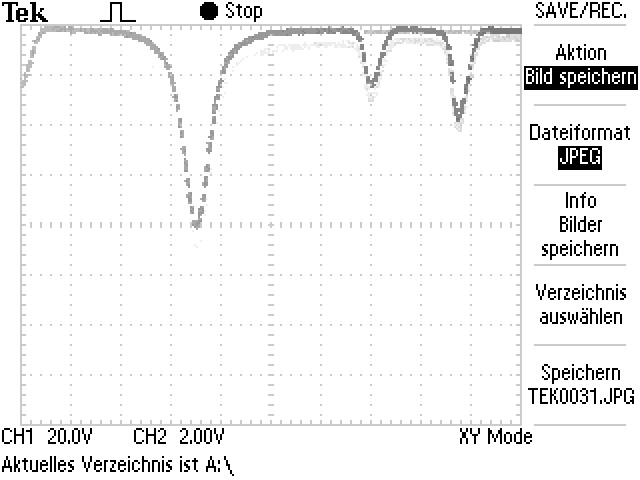
\includegraphics[height=8cm]{ressources/TEK0031.png}
  \caption{Transparenz der Zelle in Abhängigkeit von der Magnetfeldstärke bei $\nu = \SI{100}{\kilo\hertz}$.}
  \label{fig:typisch}
\end{figure}

Je nachdem wie stark das zur Resonanz gehörige Isotop vertreten ist, ist die Abnahme der Transparenz der Zelle stärker.
Somit kann über das Verhältnis der beiden Amplituden eine grobe Abschätzung für das Isotopenverhältnis getroffen werden.
In willkürlichen Einheiten können die linke Amplitude $A_1$ und die rechte Amplitude $A_2$ abgelesen werden als
\begin{align*}
  A_1 &= \input{build/A_1.tex} & A_2 &= \input{build/A_2.tex}
\end{align*}
was einem Amplituden- bzw. Isotopenverhältnis von
\begin{align*}
  \frac{A_2}{A_1} &= \input{build/A_V.tex}
\end{align*}
entspricht.
Unter der Annahme, dass die Amplitude $A_2$ zu dem Isotop $^{85}\text{Rb}$ und $A_1$ zu dem Isotop $^{87}\text{Rb}$, kann dieser Wert mit dem realen Isotopenverhältnis \cite{fuck} verglichen werden.
Diese treten mit einer Häufigkeit von
\begin{align*}
  P\left(^{85}\text{Rb}\right) &= \input{build/Rb_85.tex} & P\left(^{87}\text{Rb}\right) &= \input{build/Rb_87.tex}
\end{align*}
auf, was einem realen Isotopenverhältnis von
\begin{align*}
  \frac{P\left(^{85}\text{Rb}\right)}{P\left(^{87}\text{Rb}\right)} &= \input{build/Rb_V.tex}
\end{align*}
entspricht.

\subsection{Abschätzung des quadratischen Zeeman-Effektes}
Wie in der Theorie erläutert ergibt sich nach Gleichung \eqref{eqn:zee} eine Abweichung von der linearen Abhängigkeit vom $B$-Feld, die quadratischer Zeeman-Effekt genannt wird und bei größeren Magnetfeldern relevant wird.
Da lediglich eine grobe Abschätzung erwünscht ist, wird für das Magnetfeld der Wert $\lvert \vec{B} \rvert = \SI{250}{\micro\tesla}$ angenommen, was gerundet dem höchsten verwendeten Magnetfeld bei diesem Versuch entspricht.
Zudem mit ein Wert von $g_F = \num{0.5}$ angenommen sowie Energien für die Hyperfeinstrukturaufspaltung \cite{skript} von
\begin{align*}
  \Delta E_{\text{Hy},87} &= \SI{4.53e-24}{\joule} & \Delta E_{\text{Hy}, 85} &= \SI{2.01e-24}{\joule}
\end{align*}
für die beiden Isotope.
Werden diese Abschätzungen genutzt, ergibt sich ein Verhältnis vom linearen Term zum quadratischen Term von
\begin{align*}
  \left(\frac{U_\text{lin}}{U_\text{quad}}\right)_{87} &= \input{build/zeeman_1.tex} & \left(\frac{U_\text{lin}}{U_\text{quad}}\right)_{85} &= \input{build/zeeman_2.tex}.
\end{align*}
Somit unterscheiden sich die beiden Effekte um ca. drei Größenordnungen mit deutlich stärkerem Einfluss durch den linearen Term.

% % Examples
% \begin{equation}
%   U(t) = a \sin(b t + c) + d
% \end{equation}
%
% \begin{align}
%   a &= \input{build/a.tex} \\
%   b &= \input{build/b.tex} \\
%   c &= \input{build/c.tex} \\
%   d &= \input{build/d.tex} .
% \end{align}
% Die Messdaten und das Ergebnis des Fits sind in Abbildung~\ref{fig:plot} geplottet.
%
% %Tabelle mit Messdaten
% \begin{table}
%   \centering
%   \caption{Messdaten.}
%   \label{tab:data}
%   \sisetup{parse-numbers=false}
%   \begin{tabular}{
% % format 1.3 bedeutet eine Stelle vorm Komma, 3 danach
%     S[table-format=1.3]
%     S[table-format=-1.2]
%     @{${}\pm{}$}
%     S[table-format=1.2]
%     @{\hspace*{3em}\hspace*{\tabcolsep}}
%     S[table-format=1.3]
%     S[table-format=-1.2]
%     @{${}\pm{}$}
%     S[table-format=1.2]
%   }
%     \toprule
%     {$t \:/\: \si{\milli\second}$} & \multicolumn{2}{c}{$U \:/\: \si{\kilo\volt}$\hspace*{3em}} &
%     {$t \:/\: \si{\milli\second}$} & \multicolumn{2}{c}{$U \:/\: \si{\kilo\volt}$} \\
%     \midrule
%     \input{build/table.tex}
%     \bottomrule
%   \end{tabular}
% \end{table}
%
% % Standard Plot
% \begin{figure}
%   \centering
%   \includegraphics{build/plot.pdf}
%   \caption{Messdaten und Fitergebnis.}
%   \label{fig:plot}
% \end{figure}
%
% 2x2 Plot
% \begin{figure*}
%     \centering
%     \begin{subfigure}[b]{0.475\textwidth}
%         \centering
%         \includegraphics[width=\textwidth]{Abbildungen/Schaltung1.pdf}
%         \caption[]%
%         {{\small Schaltung 1.}}
%         \label{fig:Schaltung1}
%     \end{subfigure}
%     \hfill
%     \begin{subfigure}[b]{0.475\textwidth}
%         \centering
%         \includegraphics[width=\textwidth]{Abbildungen/Schaltung2.pdf}
%         \caption[]%
%         {{\small Schaltung 2.}}
%         \label{fig:Schaltung2}
%     \end{subfigure}
%     \vskip\baselineskip
%     \begin{subfigure}[b]{0.475\textwidth}
%         \centering
%         \includegraphics[width=\textwidth]{Abbildungen/Schaltung4.pdf}    % Zahlen vertauscht ... -.-
%         \caption[]%
%         {{\small Schaltung 3.}}
%         \label{fig:Schaltung3}
%     \end{subfigure}
%     \quad
%     \begin{subfigure}[b]{0.475\textwidth}
%         \centering
%         \includegraphics[width=\textwidth]{Abbildungen/Schaltung3.pdf}
%         \caption[]%
%         {{\small Schaltung 4.}}
%         \label{fig:Schaltung4}
%     \end{subfigure}
%     \caption[]
%     {Ersatzschaltbilder der verschiedenen Teilaufgaben.}
%     \label{fig:Schaltungen}
% \end{figure*}
